\begin{figure}[H]
	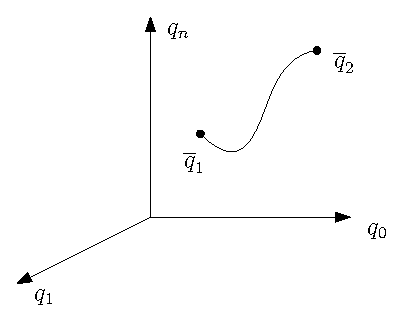
\includegraphics{8_1.eps}
\end{figure}

\begin{flalign*}
& L = L(q, \dot q, t) &\\
& \gamma = \{q(t), t \in [t_1, t_2]\; q(t_1) = q_1,\; q(t_2) = q_2\} \text{ --- какая-то траектория} &\\
& \Omega = \{q(t) \in C^2, t \in [t_1, t_2]\; q(t_1) = q_1,\; q(t_2) = q_2\} &\\
& \gamma \in \Omega &\\
\end{flalign*}

\begin{df}
Кривая, соответствующая решению уравнения Лагранжа системы с лагранжианом $L$ называется прямым путем системы. Остальные пути называются окольными.
\end{df}
\begin{ntc}
Прямой путь не единственный.
\end{ntc}
\begin{df}
$S$ --- функционал действия по Гамильтону
\[
	S = S(q(t))_{q(t) \in \Omega} = \int\limits_{t_1}^{t_2} L(q(t), \dot q(t), t) dt.
\]
\end{df}
\begin{df}
Семейство кривых $q^\varepsilon(t) = q(t, \varepsilon)^{t \in [t_1, t_2]}_{\varepsilon \in [-\varepsilon_0, \varepsilon_0]}, \; q^\varepsilon(t) \in \Omega$ --- вариация кривой $q(t)$, если 
\begin{enumerate}
\item $q(t_0) = q(t)\; \forall t \in [t_1, t_2]$,
\item $q(\varepsilon, t_1) = q_1,\; q(\varepsilon, t_2) = q_2,\; \forall \varepsilon \in [-\varepsilon_0, \varepsilon_0]$.
\end{enumerate}
\end{df}
\begin{df}
$\delta S = \left( \frac{d}{d\varepsilon}\vert_{\varepsilon = 0} S(q^\varepsilon(t)) \right)\delta \varepsilon$ --- вариация функционала $S$, соответствующая $q(t)$ при вариации $q^\varepsilon(t)$.
\end{df}

\subsection{Принцип Гамильтона}
\begin{ass}
Вариация функционала действия на некотором пути равный нулю тогда, и только тогда, когда путь прямой.
\[
	\delta S = 0\; \forall q^\varepsilon(t) \Leftrightarrow \left.\left( \frac{d}{dt}\pd{L}{\dot q} - \pd{L}{q} \right)\right|_{q = q^\varepsilon(t, 0)}
\]
\end{ass}
\begin{proof}
\begin{flalign*}
& S(q^\varepsilon(t)) = \int\limits_{t_1}^{t_2}L(q^\varepsilon(t), \dot q^\varepsilon(t), t)dt &\\
& \frac{d}{d\varepsilon}S = \int\limits_{t_1}^{t_2}\left( \pd{L}{q}\cdot \pd{q^\varepsilon}{\varepsilon} + \pd{L}{\dot q}\cdot \pd{\dot q^\varepsilon}{\varepsilon} \right)dt = \int\limits_{t_1}^{t_2} \left( \pd{L}{q}\cdot \pd{q^\varepsilon}{\varepsilon} +  \pd{L}{\dot q}\cdot \frac{d}{dt}\pd{q^\varepsilon}{\varepsilon}\right)dt = &\\ 
& = \int\limits_{t_1}^{t_2}\pd{L}{q}\cdot\pd{q^\varepsilon}{\varepsilon}dt + \left.\pd{L}{\dot q}\cdot\pd{q^\varepsilon}{\varepsilon}\right|_{t_1}^{t^2} - \int\limits_{t_1}^{t_2}\pd{q^\varepsilon}{\varepsilon}\cdot\frac{d}{dt}\pd{L}{\dot q}dt = \cancelto{0}{\left.\pd{L}{\dot q}\cdot\pd{q^\varepsilon}{\varepsilon}\right|_{t_1}^{t^2}} - \int\limits_{t_1}^{t_2}\pd{q^\varepsilon}{\varepsilon}\left( \frac{d}{dt}\pd{L}{\dot q} - \pd{L}{q} \right)dt &\\
& \left.\pd{q^\varepsilon}{\varepsilon}\right|_{\varepsilon = 0} = g(t),\; g(t_1) = g(t_2) = 0 &\\
\end{flalign*}
\begin{figure}[H]
	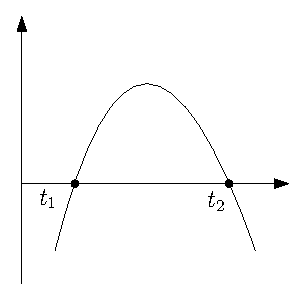
\includegraphics{8_2.eps}
\end{figure}
\begin{flalign*}
& \boxed{\Leftarrow} \quad q(t) \text{ --- прямой путь } \Rightarrow \left.\left( \frac{d}{dt}\pd{L}{\dot q} - \pd{L}{q}\right)\right|_{q = q(t)} = 0 \Rightarrow \delta S = \left.\frac{d}{d\varepsilon}\right|_{q = 0}Sd\varepsilon = 0 &\\
& \boxed{\Rightarrow} \quad \delta S = 0 \text{ при } \forall q^\varepsilon(t)\text{, пусть } \left.\left( \frac{d}{dt}\pd{L}{\dot q} - \pd{L}{q} \right)\right|_{q(t,\; 0)} = u(t) \neq 0 &\\
\end{flalign*}
\begin{flalign*}
	& f(t) = (t - t_1)(t - t_2) &\\
	& q^\varepsilon(t) = u(t)f(t)\varepsilon + q(t,\; 0) &\\
	& \delta S = - \int\limits_{t_1}^{t_2}\underbrace{u(t)f(t)}_{\left.\pd{q^\varepsilon}{\varepsilon}\right|_{\varepsilon = 0}}u(t)dt = -\int\limits_{t_1}^{t_2}(u(t), u(t))f(t)dt = 0 \Leftrightarrow u(t) = 0. \text{ Противоречие.}
\end{flalign*}
\end{proof}

\subsection{Преобразование лагранижиана при замене координат и времени}
\begin{flalign*}
	& (q,\; t) \rightarrow (\tilde q, \tilde t) \qquad \begin{cases}
		\tilde q = \tilde q(q, \;t) \\
		\tilde t = \tilde t(q, \;t) \\
	\end{cases} \qquad \det \pd{(\tilde q_1,\ldots,\tilde q_n,\; \tilde t)}{(q_1,\ldots, q_n,\; t)} \neq 0 &\\
	& \begin{cases}
		q = q(\tilde q,\; \tilde t) \\
		t = t(\tilde q,\; \tilde t) \\
	\end{cases} \qquad (1) &\\
	& L = L(q,\; \dot q,\; t) &\\
	& \tilde q' = \frac{d\tilde q}{d\tilde t} = \frac{\pd{\tilde q}{q}dq + \pd{\tilde q}{t}dt}{\pd{\tilde t}{q}dq + \pd{\tilde t}{t}dt} &\\
	& \dot q = \frac{d}{dt} = \frac{\pd{q}{\tilde q}d\tilde q + \pd{q}{\tilde t}d\tilde t}{\pd{t}{\tilde q}d\tilde q + \pd{t}{\tilde t}d\tilde t} \quad (2) &\\
	& L(q,\; \dot q,\ t) \Rightarrow \frac{d}{dt}\pd{L}{\dot q} - \pd{L}{q} = 0 \qquad (*) &\\
\end{flalign*}
\begin{ass}
	Если в уравнениях $(*)$ произвести замену $(1)$, $(2)$, то полученные уравнения будут иметь вид уравнений Лагранжа с лагранжианом
	\[
	 	\tilde L(\tilde q,\; \tilde q',\; \tilde t) = L(q,\; \dot q,\; t)|_{(1),(2)}\cdot \frac{dt}{d\tilde t}.
	 \] 
\end{ass}
\begin{proof}
	\begin{flalign*}
		& S = \int\limits_{t_1}^{t_2}L(q(t),\; \dot q(t),\; t)dt = \int\limits_{\tilde t_1}^{\tilde t_2}L(q(t),\; \dot q(t),\; t) |_{(1),(2)}\frac{dt}{d\tilde t}d\tilde t = \int\limits_{\tilde t_1}^{\tilde t_2}\tilde L(\tilde q(t),\; \tilde q'(t),\; \tilde t)d\tilde t &\\
	\end{flalign*}
\end{proof}

\begin{xmp}
	\begin{flalign*}
		& L = \frac{\dot q^2}{2},\; \tilde q = qe^{n\alpha},\; \tilde t = te^{k\alpha},\; k,\; n \in \mathbb{Z},\; \alpha \text{ --- параметр.} &\\
		& \tilde L(\tilde q,\; \tilde q',\; \tilde t) = \frac{(\tilde q'e^{(n - k)\alpha})^2}{2}\cdot e^{-k\alpha} \ovalbox{=} &\\
		& \tilde q' = \frac{d\tilde q}{\tilde t} = \frac{dq e^{n\alpha}}{dte^{k\alpha}} = \dot qe^{(n - k)\alpha},\; \dot q = \tilde q' e^{(k - n)\alpha} &\\
		& \ovalbox{=} \frac{(\tilde q')^2}{2}e^{(2k - 2n - k)\alpha} = \frac{(\tilde q')^2}{2}e^{(k - 2n)\alpha} = L(\tilde q,\; \tilde q',\; \tilde t)e^{(k - 2n)\alpha} &\\
		& \text{Если } k = 2n \text{, то } \tilde L = L(\tilde q,\; \tilde q',\; \tilde t). &\\
	\end{flalign*}
\end{xmp}

\begin{df}
	Однопараметрическое семейство преобразования координат
	\[
	 	\begin{cases}
	 		\tilde q = \tilde q(q,\; t,\; \alpha) \\
	 		\tilde t = \tilde t(q,\; t,\; \alpha) \\
	 	\end{cases} \qquad (3)
	 \] 
	называется группой вариационных симметрий системы с лагранжианом $L$, если
	\begin{enumerate}
		\item $\det \pd{(\tilde q_1,\ldots, \tilde q_n,\; \tilde t)}{(q_1,\ldots,q_n,\; t)} \neq 0$;
		\item $\tilde q(q,\; t,\; 0) = q$,\; $\tilde t(q,\; t,\; 0) = t$;
		\item $\tilde L(\tilde q,\; \tilde q', \tilde t) = L(\tilde q,\; \tilde q',\; \tilde t)$.
	\end{enumerate}
\end{df}
\begin{flalign*}
	& p = \pd{L}{\dot q},\; H = (\pd{L}{\dot q},\; \dot q) = L(q,\; \dot q,\; t),\; \eta = \left.\pd{\tilde q}{\alpha}\right|_{\alpha = 0},\; \zeta = \left.\pd{\tilde t}{\alpha}\right|_{\alpha = 0} &\\
\end{flalign*}
\begin{teo}[Эмми Нетер]
	Если $(3)$ - группа вариационных симметрий системы, то функция $f = p\eta - \zeta H$ является первым интегралом системы.
\end{teo}
\begin{xmp}
	\begin{flalign*}
		& \text{При } k = 2n:   \tilde q = qe^{n\alpha},\; \tilde t = te^{k\alpha} \text{ --- группа вариационных симметрий.} &\\
		& L = \frac{\dot q^2}{2} \qquad p = \pd{L}{\dot q} = \dot q \qquad \eta = \left.\pd{\tilde q}{\alpha}\right|_{\alpha = 0} = q e^{n\alpha}n |_{\alpha = 0} = nq &\\
		& H = p\dot q - L = \dot q^2 - \frac{\dot q^2}{2} = \frac{\dot q^2}{2}  &\\
		& \zeta = \left.\pd{\tilde t}{\alpha}\right|_{\alpha = 0} = te^{2n\alpha}\cdot 2n |_{\alpha = 0} = 2nt &\\
		& f = p\eta - \zeta H = \dot q n q - 2nt\cdot \frac{\dot q^2}{2} = n\dot q(q - \dot q t) = const &\\
		& \frac{d}{dt}\pd{L}{\dot q} - \pd{L}{q} = \ddot q = 0 \Rightarrow q = C_1t + C_2 \Rightarrow f = nC_1(C_2) = const &\\
	\end{flalign*}
\end{xmp}
\begin{xmp}
	\begin{flalign*}
		& L = L(q,\; \dot q) &\\
		& \begin{cases}
			\tilde q = q \\
			\tilde t = t + \alpha \\
		\end{cases} \text{ --- группа вариационных симметрий}
	\end{flalign*}
\end{xmp}